%------------------------------------------------------------------------------
\section{Results}
\label{sec:results}
\textbf{Kernel-level progression.} Table~\ref{tab:versions} summarizes the DP
kernel on the 1428$\times$968 image (Nsight, first seam).
\textbf{\emph{Fused}} is the structural baseline; \textbf{\emph{GridSync}}
regresses (barrier-bound); \textbf{\emph{Prefetch}} removes the dominant
\texttt{long\_scoreboard} stall and gives the \textbf{largest single jump}
(\textbf{1.67$\times$}); \textbf{\emph{BytePtr}} trims store traffic to reach
the latency floor.

% Table I — DP kernel duration per configuration
% Protocol: Nsight Compute, first seam, 1428×968 (Broadway)
% Note: Prefetch and BytePtr speedups (1.67× and 1.85×) are consistent 
% across resolutions (1920×1080: 1.96× and 2.08×; 960×540: 1.95× and 1.97×).
\begin{table}[t]
\caption{DP kernel per configuration (1428$\times$968, Nsight, first seam).
\emph{Naive} uses $H$ per-row launches; no single fused kernel to profile.
Prefetch/BytePtr improvements verified consistent across standard resolutions.}
\label{tab:versions}
\centering
\begin{tabular}{@{}lcc@{}}
\toprule
\textbf{Method} & \textbf{Duration (ms)} & \textbf{vs \emph{Fused}} \\
\midrule
\emph{Naive}     & ---            & ---                        \\
\emph{Fused}     & 1.46           & 1.00$\times$ (baseline)    \\
\emph{GridSync}  & \textbf{1.66}  & \textbf{0.88$\times$} (regressed) \\
\emph{Prefetch}  & \textbf{0.872} & \textbf{1.67$\times$}      \\
\emph{BytePtr}   & 0.790          & 1.85$\times$               \\
\emph{Templated} & 0.790          & 1.85$\times$               \\
\bottomrule
\end{tabular}
\end{table}


\textbf{Hardware footprint (Table~\ref{tab:hw}).}
\emph{Fused} and \emph{GridStride} store the full $W$-wide cost row in
shared memory ($5W$ bytes), which reaches 37.5\,KB at 8K yet still fits
within the 96\,KB limit.
\emph{Tiled}'s per-block shared memory is fixed at 0.9\,KB regardless of
$W$ (from Eq.~\eqref{eq:shmem}), enabling 60 independent blocks to coexist
with negligible resource pressure.
Register counts decrease from \emph{Fused} (${\approx}$20) to \emph{Tiled}
(${\approx}$16): \emph{Tiled}'s per-strip loop has fewer live variables than
the CPT-unrolled single-block design.

% Table III — Kernel hardware footprint (transposed: methods as columns)
% Register counts from Nsight Compute; shmem calculated from kernel structure.
% Fused/GridStride shmem = 5W bytes (2×ping-pong int16 + back-ptr int8 per row).
% Tiled shmem = 5(S+2T) bytes from Eq.(3), constant regardless of W.
\begin{table}[t]
\caption{Kernel hardware footprint (register counts from Nsight Compute;
shared memory calculated from kernel structure).
\emph{Fused}/\emph{GridStride} shared memory scales with $W$;
\emph{Tiled}'s 0.9\,KB/block is independent of $W$ (Eq.~\eqref{eq:shmem}).}
\label{tab:hw}
\centering
\begin{tabular}{@{}lccc@{}}
\toprule
 & \emph{Fused} & \emph{GridStride} & \textbf{\emph{Tiled}} \\
 & (1428\,px) & (8K wide) & (8K wide) \\
\midrule
Reg / thread   & ${\approx}20$ & ${\approx}18$ & ${\approx}16$ \\
Shmem / block  & 7.0\,KB       & 37.5\,KB      & \textbf{0.9\,KB} \\
Active SMs     & 1             & 1             & \textbf{60} \\
\bottomrule
\end{tabular}
\end{table}


\textbf{End-to-end throughput.} Table~\ref{tab:fullresults} gives
whole-pipeline ms/seam for CPU (a single core and the best multicore OpenMP
configuration), \emph{Naive} GPU, the prior single-block best (\emph{Templated} at ${\le}4$K;
\emph{GridStride} at 6K--8K), and \emph{Tiled}.
All rows use the same 50-seam best-of-3 protocol.
Key observations:
\textbf{(1)} At ctrl--4K, \emph{Tiled} beats \emph{Templated} by
\textbf{$1.13$--$1.43\times$} while remaining bit-exact.
\textbf{(2)} At 6K/8K, \emph{Tiled} is \textbf{$2.6\times$} and
\textbf{$3.1\times$} faster than the prior best (\emph{GridStride}).
\textbf{(3)} Over the best multicore CPU baseline (NUMA-aware OpenMP, best of
1--32 threads; Appendix~\ref{app:omp}), \emph{Tiled}'s speedup grows
\emph{monotonically} from \textbf{3.6$\times$} (ctrl) to \textbf{6.2$\times$}
(8K)---larger images engage more of the 60\,SMs. Over a single CPU core the
range is \textbf{16$\times$}--\textbf{57$\times$}.
\textbf{(4)} Kim~et~al.~\cite{kim2015} found their \emph{exact} single-GPU DP
reached only $5.9{\times}$ on their earlier-generation hardware and abandoned
it for the approximate NCSC heuristic. Hardware differs, so this is a
\emph{design}-level point, not a normalized comparison: latency hiding makes
the exact DP they discarded scale well, removing the need to approximate.

% Table II — Full end-to-end ms/seam across all methods and resolutions
% Protocol: wall-clock, best-of-3, 50 seams
% † Templated fails at ≥6K (register overflow)
% ‡ CPU best: best ms/seam over 1–32 threads, NUMA-aware OpenMP (v4), see Appendix D
% Fused ctrl not benchmarked (single-block fits 540-row images but was not collected)
% GridStride: only benchmarked at 2K, 6K, 8K
\begin{table*}[t]
\caption{End-to-end ms/seam across all methods and resolutions (best-of-3, 50 seams).
\textbf{Bold} = best GPU result per resolution.
$\dagger$\emph{Templated} fails at ${\ge}6$K (register file overflow at CPT\,=\,8).
--- indicates not benchmarked or unsupported at that resolution.
$\ddagger$ \emph{CPU best} is the best ms/seam over 1--32 threads of our
NUMA-aware OpenMP baseline (persistent team, parallel first-touch, cache
ping-pong); the optimum lies at 8--32 threads (Appendix~\ref{app:omp}).}
\label{tab:fullresults}
\centering
\begin{tabular}{@{}lcccccc@{}}
\toprule
\textbf{Method} & \textbf{ctrl} & \textbf{1080p} & \textbf{2K} & \textbf{4K} & \textbf{6K} & \textbf{8K} \\
 & {\scriptsize 960$\times$540} & {\scriptsize 1920$\times$1080} & {\scriptsize 2560$\times$1440} & {\scriptsize 3840$\times$2160} & {\scriptsize 6144$\times$3456} & {\scriptsize 7680$\times$4320} \\
\midrule
CPU 1 core                   & 5.00  & 21.6  & 37.5  & 83.6  & 212   & 325   \\
CPU best$^\ddagger$          & 1.14  & 3.59  & 5.63  & 9.88  & 25.6  & 35.4  \\
\midrule
\emph{Naive}                 & 1.37  & 3.10  & 3.77  & 5.92  & 10.3  & 13.9  \\
\emph{Fused}                 & ---   & 1.94  & 3.08  & 6.73  & 12.63 & 21.3  \\
\emph{Templated}$\dagger$    & 0.355 & 1.08  & 1.57  & 3.10  & ---   & ---   \\
\emph{GridStride}            & ---   & ---   & 2.87  & ---   & 10.8  & 17.7  \\
\textbf{\emph{Tiled}} (ours) & \textbf{0.314} & \textbf{0.917} & \textbf{1.25} & \textbf{2.16} & \textbf{4.16} & \textbf{5.73} \\
\midrule
\emph{Speedup vs 1 core}     & 16$\times$ & 24$\times$ & 30$\times$ & 39$\times$ & 51$\times$ & \textbf{57$\times$} \\
\emph{Speedup vs CPU best}   & 3.6$\times$ & 3.9$\times$ & 4.5$\times$ & 4.6$\times$ & 6.2$\times$ & \textbf{6.2$\times$} \\
\bottomrule
\end{tabular}
\end{table*}


\textbf{Scaling in pixels (Fig.~\ref{fig:scaling}).}
\emph{Tiled}+Prefetch grows sublinearly: a 64$\times$ increase in pixels
(ctrl$\to$8K) costs only ${\sim}18\times$ more time
(0.314$\to$5.73\,ms/seam). Its slope is consistently below \emph{Templated}'s
on images where both run.

\begin{figure}[t]
\centering
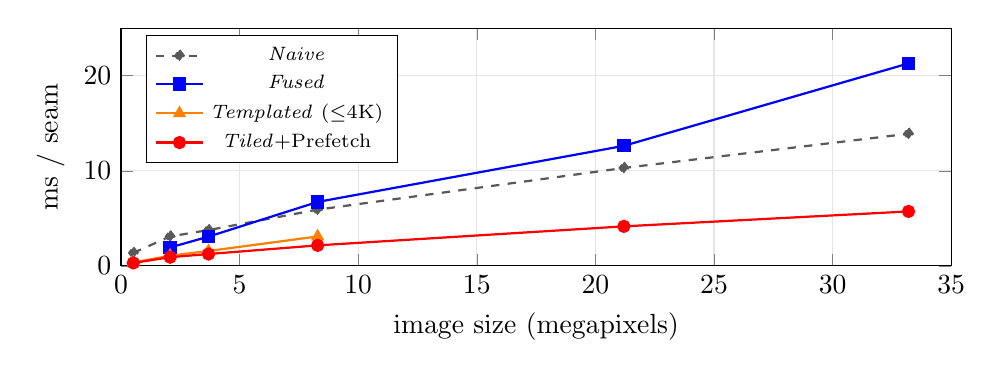
\begin{tikzpicture}
\begin{axis}[
  width=\columnwidth, height=4.6cm,
  xlabel={image size (megapixels)}, ylabel={ms / seam},
  xlabel near ticks, ylabel near ticks,
  xmin=0, xmax=35, ymin=0, ymax=25,
  legend pos=north west, legend style={font=\scriptsize},
  grid=major, grid style={gray!20},
  xtick={0,5,10,15,20,25,30,35},
]
% Naive: ctrl, 1080p, 2K, 4K, 6K, 8K (baseline: H launches, global R/W)
\addplot[mark=diamond*,gray!70!black,thick,dashed]
  coordinates {(0.52,1.37)(2.07,3.10)(3.69,3.77)(8.29,5.92)(21.2,10.3)(33.2,13.9)};
% Fused: 1080p, 2K, 4K, 6K, 8K (single-block, shared-mem ping-pong)
\addplot[mark=square*,blue,thick]
  coordinates {(2.07,1.94)(3.69,3.08)(8.29,6.73)(21.2,12.63)(33.2,21.3)};
% Templated: ctrl, 1080p, 2K, 4K (fails at 6K/8K, register overflow)
\addplot[mark=triangle*,orange,thick]
  coordinates {(0.52,0.355)(2.07,1.08)(3.69,1.57)(8.29,3.10)};
% Tiled+Prefetch: ctrl, 1080p, 2K, 4K, 6K, 8K
\addplot[mark=*,red,thick]
  coordinates {(0.52,0.314)(2.07,0.917)(3.69,1.25)(8.29,2.16)(21.2,4.16)(33.2,5.73)};
\legend{\emph{Naive}, \emph{Fused}, \emph{Templated} (${\le}4$K), \emph{Tiled}+Prefetch}
\end{axis}
\end{tikzpicture}
\caption{ms/seam vs.\ image size (0.52--33.2\,MP). \textbf{\emph{Tiled}+Prefetch}
has the lowest slope at all sizes and reaches \textbf{57$\times$} over CPU at 8K.
\emph{Templated} stops at 4K (register overflow). The gap to \emph{Fused}
widens with image size.}
\label{fig:scaling}
\end{figure}
